\documentclass{article}
\usepackage[utf8]{inputenc}
\usepackage{amsmath}
\usepackage{amsthm}
\usepackage{amsfonts}
\usepackage{amssymb}
\usepackage{amstext}
\usepackage{gensymb}
\usepackage{graphicx}
%\usepackage{bbold}
%\usepackage{url}
%\usepackage{booktabs}
%\usepackage{marvosym}
%\usepackage{wasysym}
\pagenumbering{arabic}
\usepackage{fancyhdr}
\usepackage[margin=1.0in]{geometry}
\usepackage{eucal}
\usepackage{multicol}
\usepackage{verbatim}
\usepackage{adjustbox}

\pagestyle{fancy}
\fancyhf{}
\rhead{MATH 6250}
\lhead{Alexander Winkles}
\chead{\Large \textbf{Homework 4}}
\cfoot{Page \thepage}

\begin{document}

Work for many problems were omitted when typing in \LaTeX.

\begin{enumerate}

\item \textit{Problem 1}\\
\begin{enumerate}
\item Without loss of generality, begin by taking one point to be (0,0,1) and the other to be $(\sin(u_0),0,\cos(u_0))$.
To prove that the shortest path between two points on the unit sphere is an arc of a great circle, let $\alpha(t) = (\sin(u(t))\cos(v(t)),\sin(u(t))\sin(v(t)),\cos(u(t)))$, with $a \leq t \leq b$.
From this, we know that $u(a) = 0, v(a) = 0, u(b) = u_0, v(b) = 0$. 
Begin by taking the derivative of $\alpha(t)$.
This is equal to 
\begin{equation*}
\alpha'(t) = (\cos(u)\cos(v)*u' - \sin(u)\sin(v)*v', \cos(u)\sin(v)*u' + \sin(u)\cos(v)*v', -\sin(u)*u')
\end{equation*}
Taking the magnitude of this and then reducing it to its simpliest form yield:
\begin{equation*}
|\alpha'(t)| = \sqrt{(u')^2+(v')\sin^2(u)}
\end{equation*}
Notice that when $v(t) = 0$, which implies $v'(t) = 0$, it can be seen that $|\alpha'(t) = u'$.
Since $(v')^2\sin^2(u) \geq 0$, it is easy to see that 
\begin{equation*}
\displaystyle\int_a^b u' dt \leq \displaystyle\int_a^b \sqrt{(u')^2+(v')^2\sin^2(u)} dt
\end{equation*}
When $v(t) = 0$, it is implied that the arc is a great circle, so thus the statement is true. \qed

\item Begin by noting that if taking the dot product of P and Q gives $P \cdot Q = |P||Q|\cos^{-1}(\Theta)$. 
Since these points are on the unit sphere, their magnitudes are equal to 1. 
Rearranging this shows $\arccos(P \cdot Q) = \Theta$.
The points in question are on the unit sphere, and all have magnitudes of 1, as said above.
This means 

\end{enumerate}

\item \textit{Problem 2}\\
This is a closed plane curve with $\kappa>0$ that is not convex.
\begin{center}
\adjustbox{valign=t}{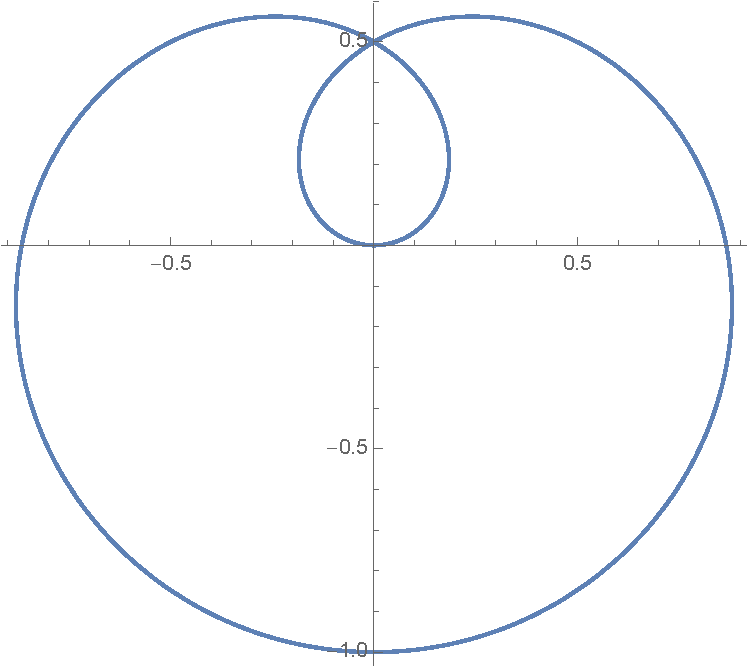
\includegraphics[width=10cm]{rose}}
\end{center}

\item \textit{Problem 4}\\

From Theorem 3.5 of the text, we know that $\displaystyle\int_C \kappa ds = \pm 2\pi$.
We also know that $\kappa \leq c$. 
Likewise $\displaystyle\int_0^L c ds = L\cdot c$
From the inequality, $2\pi =\displaystyle\int_0^L \kappa ds \leq \displaystyle\int_0^L c ds = L \cdot c$.
Thus, when rearranged, $\frac{2\pi}{c} \leq L$, as desired. \qed

\item \textit{Problem 6}\\
Crofton's Formula states that the length of a spherical curve $\gamma$ is given by $\pi \cdot$(Average number of lines that cross $\gamma$ in a given direction).
From the problem, we know the curve has a constant breadth of $\mu$ for any line through its center.
Thus, the average number of lines that cross $\gamma$ from any direction is $\displaystyle\int_0^{\mu} 1 dt = \mu$.
This gives us $length(\gamma) = \pi\mu$.

\item \textit{Problem 7}\\

\begin{enumerate}

\item Assume that the line given is tangent. 
From this, we know that $\left< \alpha', (\cos\theta,\sin\theta)\right> = 0$.
We also know that $\left< \alpha, (\cos\theta,\sin\theta)\right> = p(\theta)$.
Taking the derivative of this gives $\left< \alpha',(\cos\theta,\sin\theta)\right> + \left< \alpha, (-\sin\theta,\cos\theta)\right> = p'(\theta)$, where the first term is zero.
A linear system can now be established and solved:
\begin{equation*}
\begin{bmatrix}
\cos\theta & \sin\theta\\
-\sin\theta & \cos\theta
\end{bmatrix}
\begin{bmatrix}
x \\
y
\end{bmatrix}
=
\begin{bmatrix}
p(\theta)\\
p'(\theta)
\end{bmatrix}
\end{equation*}
By taking the inverse of this, we obtain:
\begin{equation*}
\begin{bmatrix}
x\\
y
\end{bmatrix}
=
\begin{bmatrix}
\cos\theta & -\sin\theta\\
\sin\theta & \cos\theta
\end{bmatrix}
\begin{bmatrix}
p(\theta)\\
p'(\theta)
\end{bmatrix}
\end{equation*}
Multiplying this out gives the equation provided in problem, proving the statement. \qed

\item We know what $\alpha$ equals from the problem above. 
Now, we find $\alpha'$ and $\alpha''$, which are:
\begin{align*}
\alpha' &= (-\sin\theta(p(\theta)+p''(\theta)),\cos\theta(p(\theta)+p''(\theta)))\\
\alpha'' &= (-\cos\theta(p(\theta)+p''(\theta))-\sin\theta(p'(\theta)+p'''(\theta)), -\sin\theta(p(\theta)+p''(\theta))+\cos\theta(p'(\theta)+p'''(\theta))).
\end{align*}
From class, we know the generalize formula for curvature to be 
\begin{equation*}
\kappa = \frac{|\alpha' \times \alpha''|}{|\alpha'|^3}.
\end{equation*}
Calculating the magnitude of the cross product gives $(p(\theta)+p''(\theta))^2$, where calculations were omitted for the sake of typing in \LaTeX.
Likewise, with calculations omitted, $|\alpha'|^3 = (p(\theta)+p''(\theta))^3$, so by the formula above $\kappa = \frac{1}{p(\theta)+p''(\theta)}$.
\qed

\item We know that arclength is equal to the integral of the magnitude of the derivative of $\alpha$. 
$|\alpha'| = p(\theta)+p''(\theta)$, which is seen easily. 
Thus, 
\begin{equation*}
L = \displaystyle\int_0^{2\pi} (p(\theta)+p''(\theta))d\theta = \displaystyle\int_0^{2\pi} p(\theta) d\theta + \displaystyle\int_0^{2\pi} p''(\theta) d\theta
\end{equation*}
But, $\displaystyle\int_0^{2\pi} p''(\theta) = p'(\theta)|_0^{2\pi}$.
Evaluating this integral results in $p'(\theta) = 0$ for the range, so $L = \displaystyle\int_0^{2\pi} p(\theta)$. \qed

\item I believe you need to use Stoke's theorem for this, but did not manage to attempt it before the due date.

\item

\end{enumerate}

\item \textit{Problem 8}\\

\begin{enumerate}

\item Let $\mathbf{X} = \cos\theta\mathbf{N} + \sin\theta\mathbf{B}$. 
Taking its cross product with \textbf{T}, we find $\mathbf{T}\times\mathbf{X} = \cos\theta\mathbf{B} - \sin\theta\mathbf{N}$. 
Now, $\mathbf{X'} = -\sin\theta\mathbf{N} + \cos\theta(-\kappa\mathbf{T} + \tau\mathbf{B}) + \cos\theta\mathbf{B} - \sin\theta\tau\mathbf{N}$. 
Dotting this with the resulting cross product gives $\mathbf{X'}\cdot(\mathbf{T}\times\mathbf{X}) = 1 + \tau$.
Thus, 
\begin{equation*}
tw(C,\mathbf{X}) = \frac{1}{2\pi}\displaystyle\int_0^L (1+\tau) ds.
\end{equation*}
Note that if \textbf{X} and \textbf{X*} are two unit normal fields, then the difference in their twist can be accounted for by extra bit of rotation.

\item

\item

\end{enumerate}

\item \textit{Additional Problem}\\
Already, we know that $\mathbf{T'} =\kappa\mathbf{N}, \mathbf{N'} = -\kappa\mathbf{T} + \tau\mathbf{B}, \mathbf{B'} = -\tau\mathbf{N}$. 
Let $w(s) = a\mathbf{T} + b\mathbf{N} + c\mathbf{B}$.
By taking cross products, using the fact that $(a + b)\times c = a \times c + b \times c$, we find that
\begin{align*}
w(s) \times \mathbf{T} &= -b\mathbf{B} + c\mathbf{N}\\
w(s) \times \mathbf{N} &= a\mathbf{B} - c\mathbf{T}\\
w(s) \times \mathbf{B} &= -a\mathbf{N} + b\mathbf{T}
\end{align*}
Matching these to the known equations, it is easy to see that $w(s) = \tau\mathbf{T} + \kappa\mathbf{B}$, with a length of $\sqrt{\tau^2 + \kappa^2}$.

\item \textit{Graduate Problem}\\

Suppose we have a polygon in space, V, with vertices.
Connect all of the adjacent vertices with one another and a point p to form the ``cone of V to p".

\begin{enumerate}

\item Let p be inside the convex hull of polygon V. 
Have some plane cut through point p, and notice that there will be parts of the polygon on each side perpendicular to the plane.
Since V is a closed space curve, and it is found in both the northern and southern hemispheres of a sphere with the plane cutting through it, it can be seen that the intrinsic cone angle $\theta(p) \geq 2\pi$.

\item As you take p outside of the convex hull and move it very far away from p, the intrinsic cone angle will gradually decrease until its limit is zero.
Thus, by the intermediate value theorem, since inside that convex hull the angle is greater than or equal to $2\pi$ and infinitely far away is it approximately zero, there is some point $p_0$ in between 
where the angle is $2\pi$ exactly.

\item Now we will construct a planar polygon V* by taking the triangles formed with the vertices and $p_0$ and laying them a plane about the origin.
This act is a rigid motion, and thus all lengths and angles are preserved. 
Since we chose the point $p_0$ have an intrinsic cone angle of $2\pi$, when we place all of the triangles together their polygon will be closed.

\item In problem (1b), we showed that the shortest path between two points was the line that connects them directly.
Take the planar polygon V* and connect two points on it with a line that are not vertices. 
Fold the polygon back into its spacial form V, and notice that the shortest path between two points is not the line drawn, but the one that is directly connecting them.
Thus, $|V(s)-V(t)| \leq |V*(s) - V*(t)|$. 
This can easily be extended to smooth curves, because the direct path will be shorter or eqivalent in space to the path in the plane, regardless of how smooth the curve is. \qed

\end{enumerate}

\end{enumerate}

Problems were collaborated on with Hollis Neel.

\end{document}
